\section{Illustrative Visualisation}
Computer supported interactive and expressive visualisations through abstractions as in traditional illustrations.

Illustrative visualisation uses server \emph{non-photorealistic rendering} (NPR) techniques:
\begin{itemize}
    \item Smart visibility
    \item Silhouettes
    \item Hatching (shading based on stroke density)
    \item Tone Shading
    \item Focus and Context techniques
    
    Context-reserving volume rendering.
\end{itemize}

\subsection{Smart Visibilty}
\begin{itemize}
\item Cut-aways
\item Ghosted views
\item Section views
\item Exploded views
\item Browsing Deformations:
    \begin{itemize}
        \item Leafer
        \item Peeler
    \end{itemize}
\end{itemize}

\subsection{Silhouette Algorithms}
The \emph{silhouette} of a surface consists of these points where the view vector $V$ and surface normal $N$ are orthogonal.

Silhouettes can be either \emph{outlines} or \emph{internal silhouettes}.


In contrast to other important feature lines such as curvature ridges/valleys and texture boundaries, silhouettes are view-dependent.

 \paragraph{Object Space Algorithms} exist for:
 \begin{description}
 \item Polygonal surfaces
 
     For each polygon
     \begin{itemize}
         \item Set Front-Facing flag to all edges if $N\cdot V \geq 0$
         \item Set Back-Facing flag to all edges if $N\cdot V<0$
     \end{itemize}
     for each edge draw if both flags are set.

 \item Implicit surfaces
 \item NURBS surfaces
 \end{description}
\paragraph{Image Space Algorithms} exist for:
\begin{description}
\item Polygonal Surfaces:
    \begin{itemize}
    \item Render polygons with depth buffer enabled
    \item Look for discontinuities in depth buffer:
        \begin{itemize}
            \item Compute depth difference between to adjacent pixels, or the Laplacian on a $3\times 3$ stencil.
            \item If larger than the threshold, draw a silhouette pixel.
        \end{itemize}
    \end{itemize}
\item Volume Data (Ebert and Rheingans):
    
    Idea: "Silhouette points" are where the gradient is orthogonal to the view vector. Use an opacity transfer function depending on $|\nabla s \cdot V|$.
\end{description}


\subsubsection{Hatching}
Volume illustration with hatching:
\begin{itemize}
\item Compute an isosurface
\item Compute \emph{curvature fields} ($1^{st}$ and $2^{nd}$ principal curvature directions on the isosurface), fast algorithm by Monga et al. 
\item Compute hatching as streamlines of both curvature fields using \emph{streamline placement techniques}.
\end{itemize}

\subsection{Illuminated Streamlines}
Phong's local lightimg model
\begin{align*}
     I= I_\text{ambient} + I_\text{diffuse} + I_\text{specular} = k_a +k_d L\cdot N+k_s(V\cdot R)^n
\end{align*}
requires a \emph{normal vector} which for a curve in space is underspecified.

\subsubsection{Maximum Principle}
[Banks]
\begin{itemize}
    \item Diffuse reflection is computed using the rotation angle which gives a maximum value.
    \item Specular reflection is computed using the rotation angle which gives a maximum value (a different angle in general!)
    \item Implemented with OpenGL texture mapping.
\end{itemize}

\subsubsection{Cylinder Averaging}
[Schussmann]

Diffuse and specular reflection are compute as average over the part of a cylinder which is both \emph{visible} and \emph{lit}.

Implemented as a fragment shader.

\begin{figure}[H]
\centering
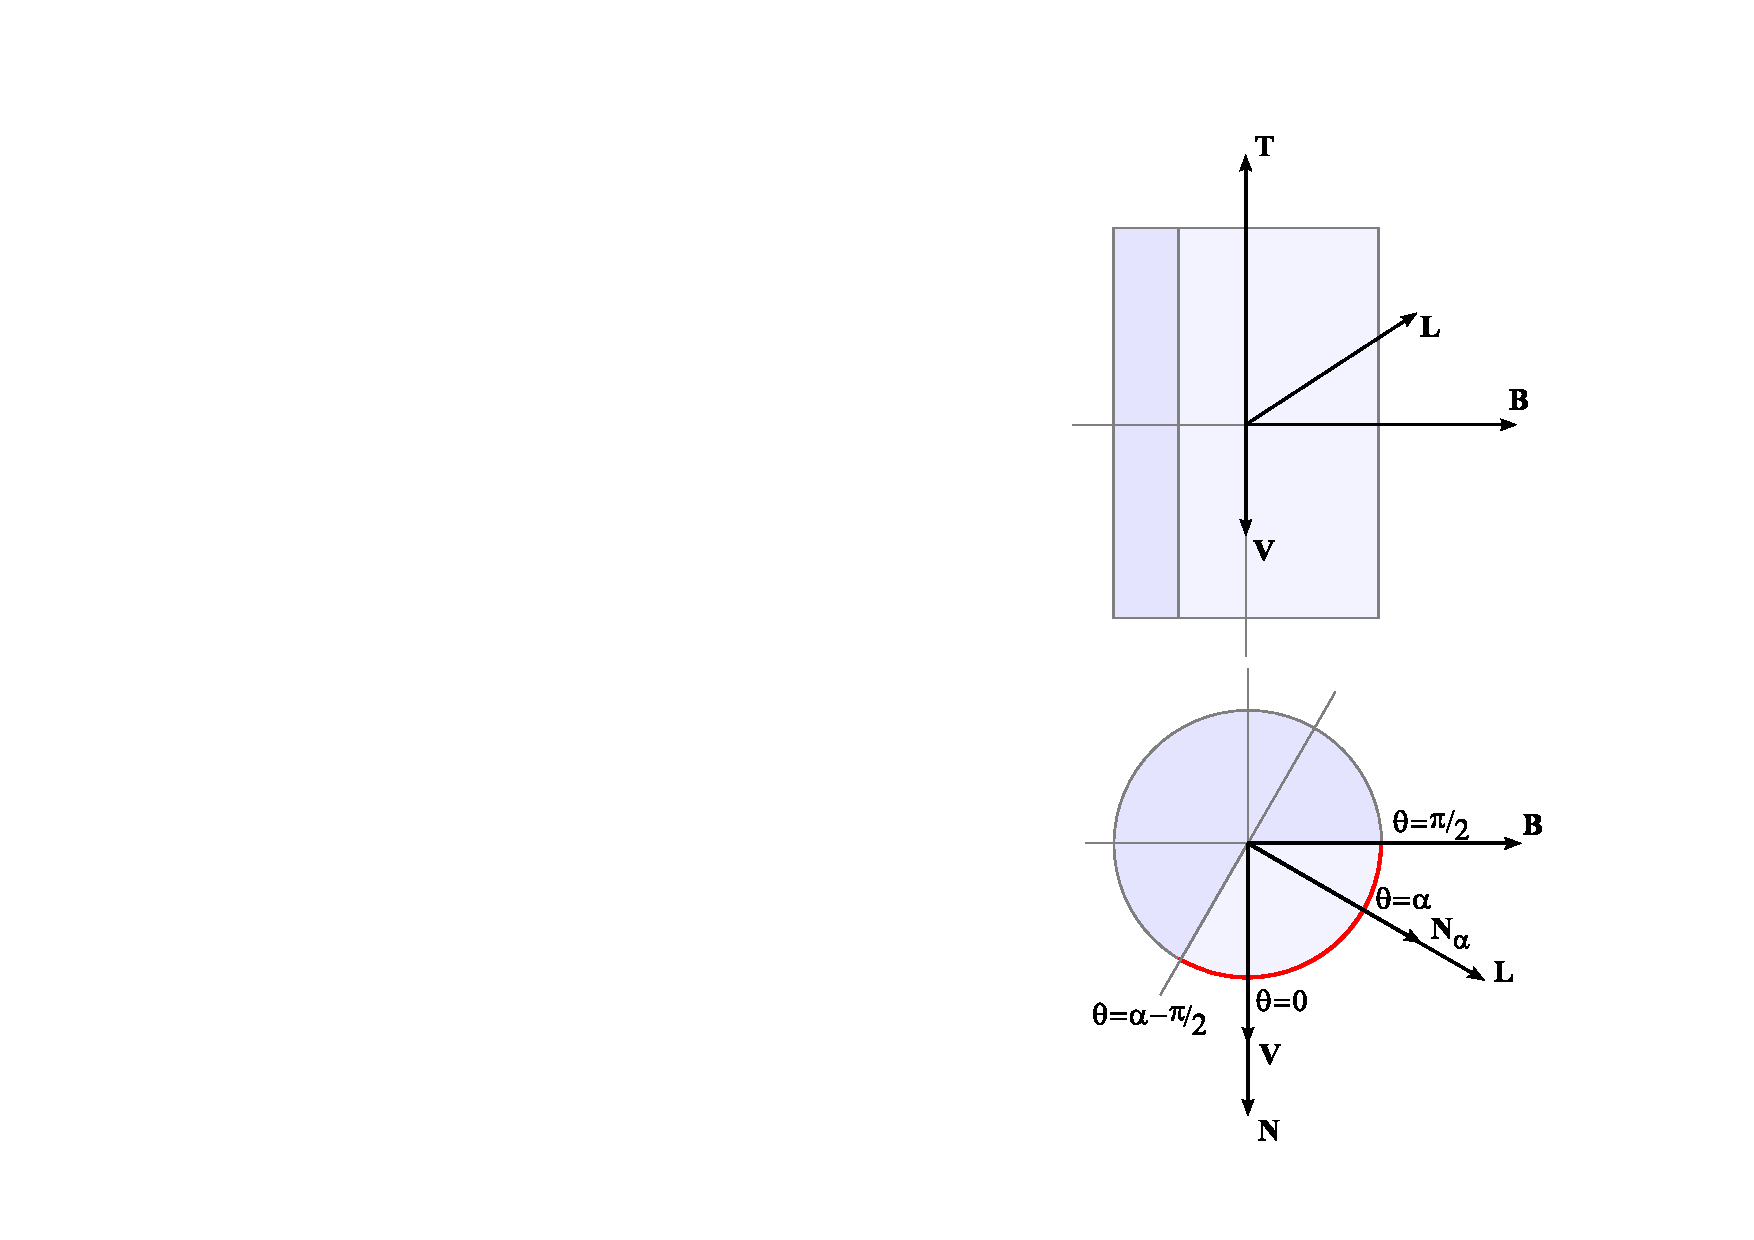
\includegraphics[width=0.4\textwidth,page=1]{img/11_illuminated_streamlines}
\end{figure}

Example: Horizontal sine curves vertically stacked:
\begin{figure}[H]
\centering
\includegraphics[width=0.4\textwidth,page=2]{img/11_illuminated_streamlines}
\end{figure}

The comparison shows: Maximum principle works well only for specular diffusion.

\subsection{Tone Shading}
\emph{Tone shading} or "toon shading" uses \emph{tones} instead of \emph{luminance} for shading.

\begin{figure}[H]
\centering
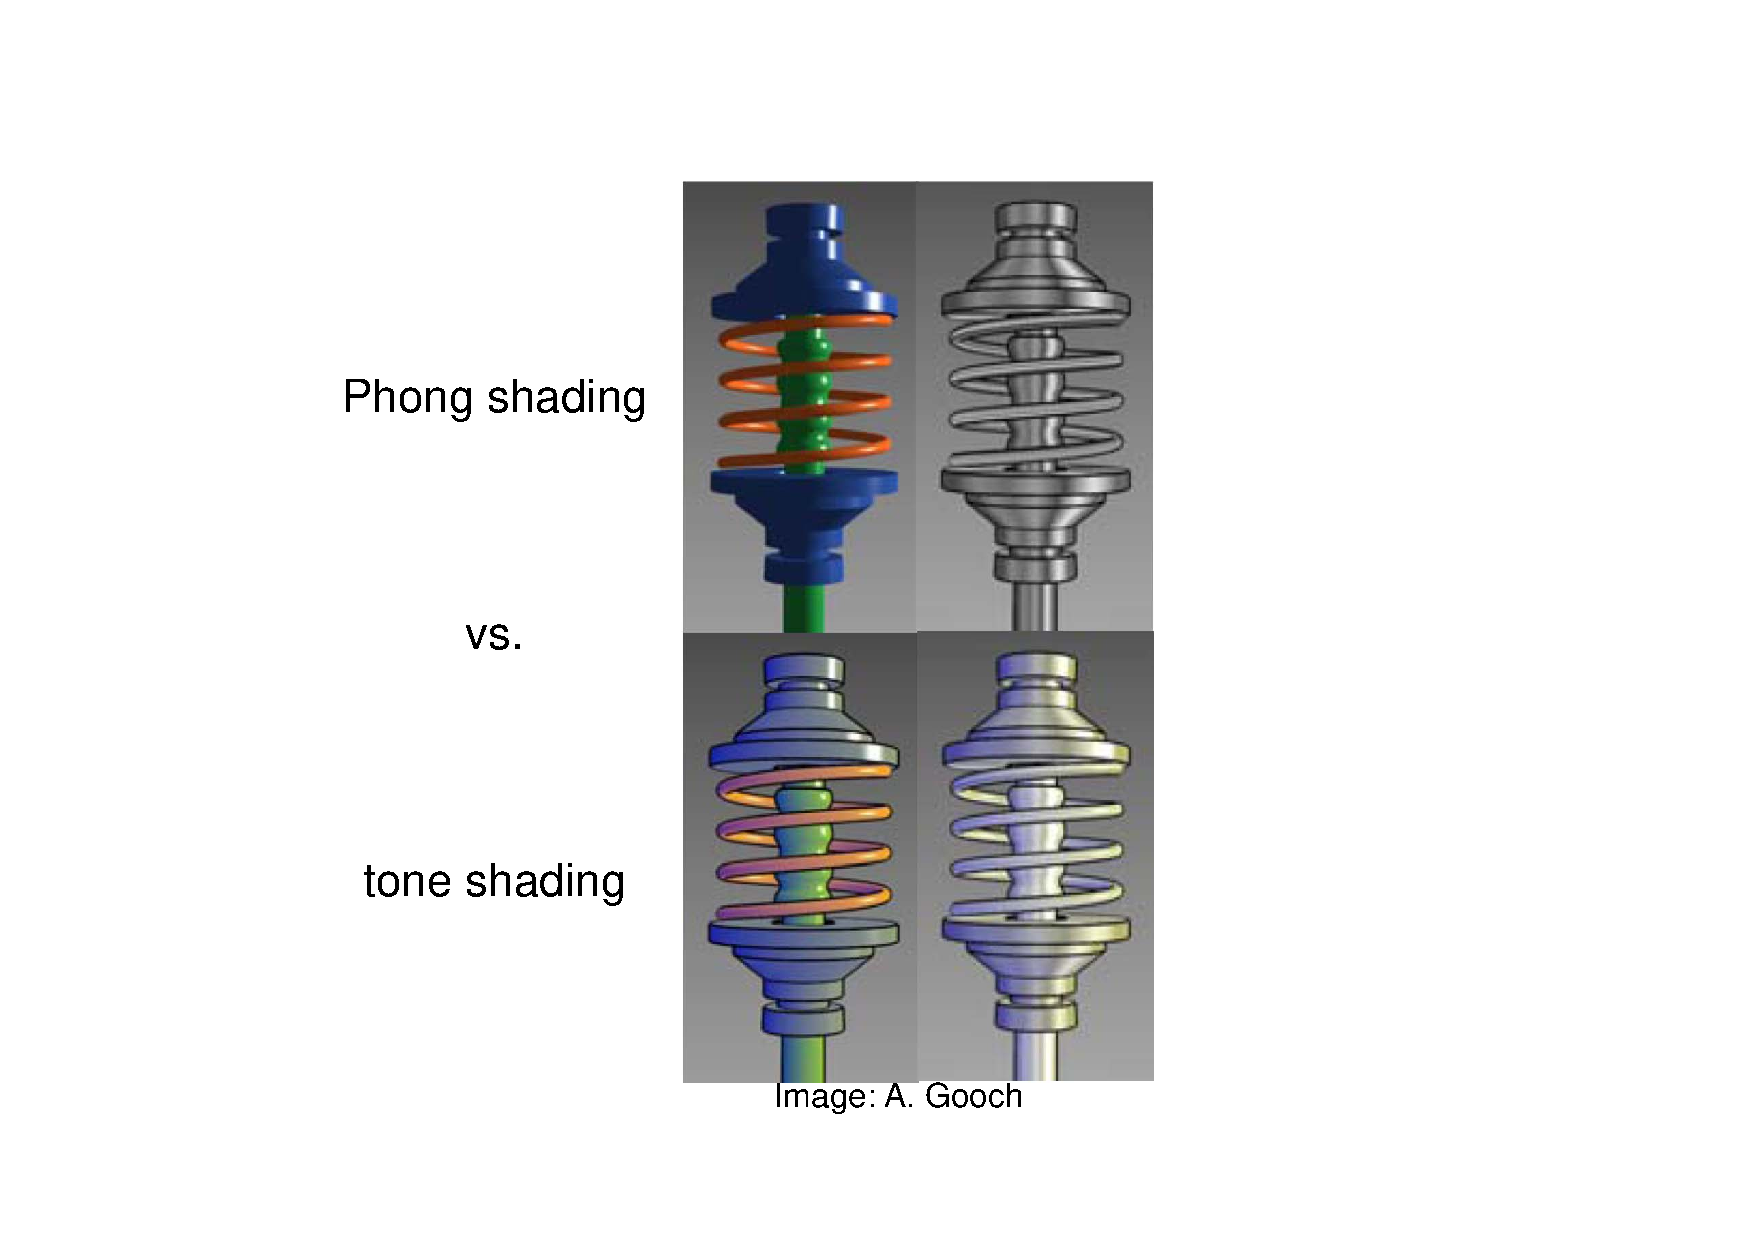
\includegraphics[width=0.7\textwidth]{img/11_tone_shading}
\end{figure}

\begin{itemize}
\item Use Warm to cool hue shift
\item Depth cue: Warm colours advance while cool colours recede.
\end{itemize}

\subsection{Context-Preserving Volume Rendering}
Ghosted view: Surface transparency depends on the \emph{grazing angle} (angle between view ray and surface). 

More transparent for a large, more opaque for a small grazing angle. 

Context-preserving volume rendering (Bruckner):
 Use of ghosted views in Volume rendering:
\begin{figure}[H]
\centering
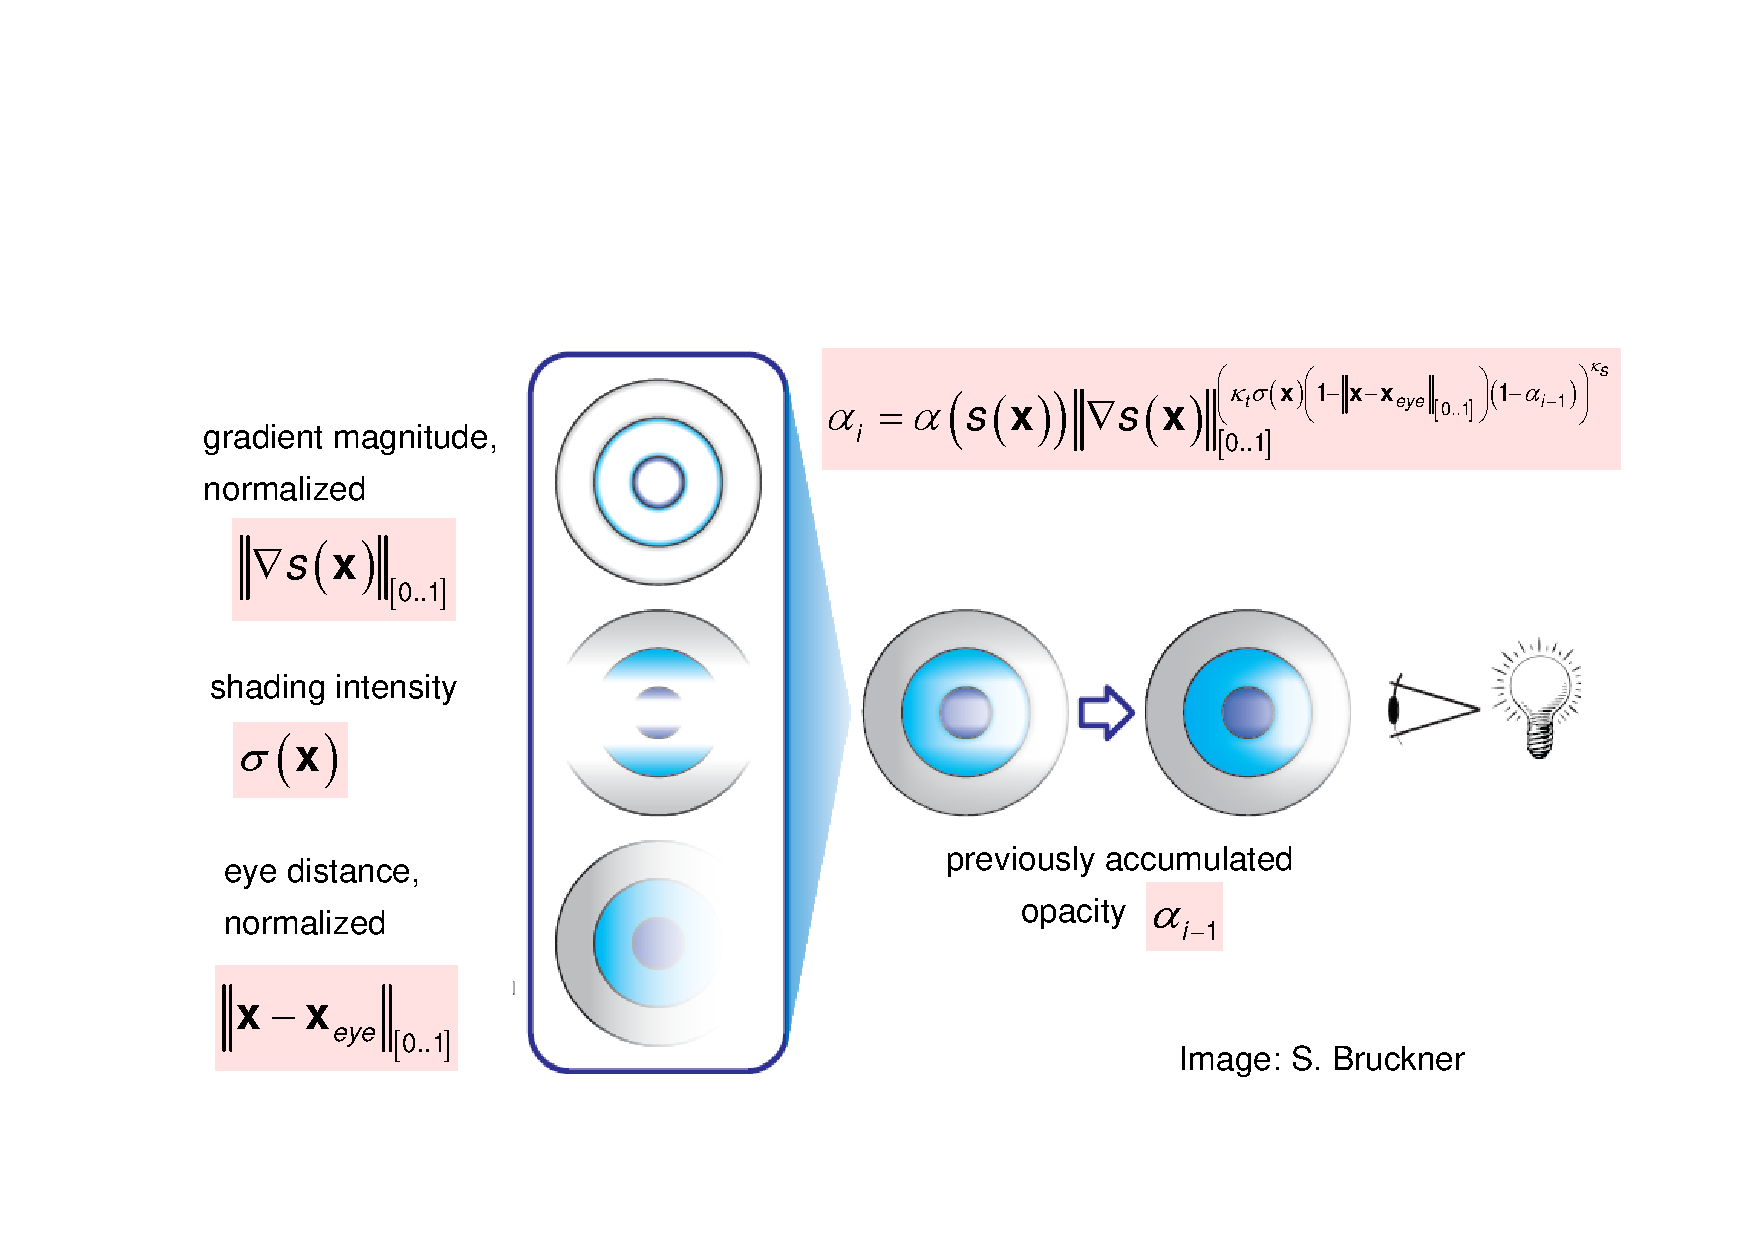
\includegraphics[width=0.8\textwidth,page=1]{img/11_bruckner}
\end{figure}

Parameters:
\begin{description}
\item $k_t$ corresponds roughly to the depth of a clipping plane.
\item $k_s$ controls the sharpness of the transition between visible and clipped.
\end{description}

\subsection{Illustrative Visualisation of (Flow) Surfaces}
Transparency methods for surface rendering:
\begin{figure}[H]
\centering
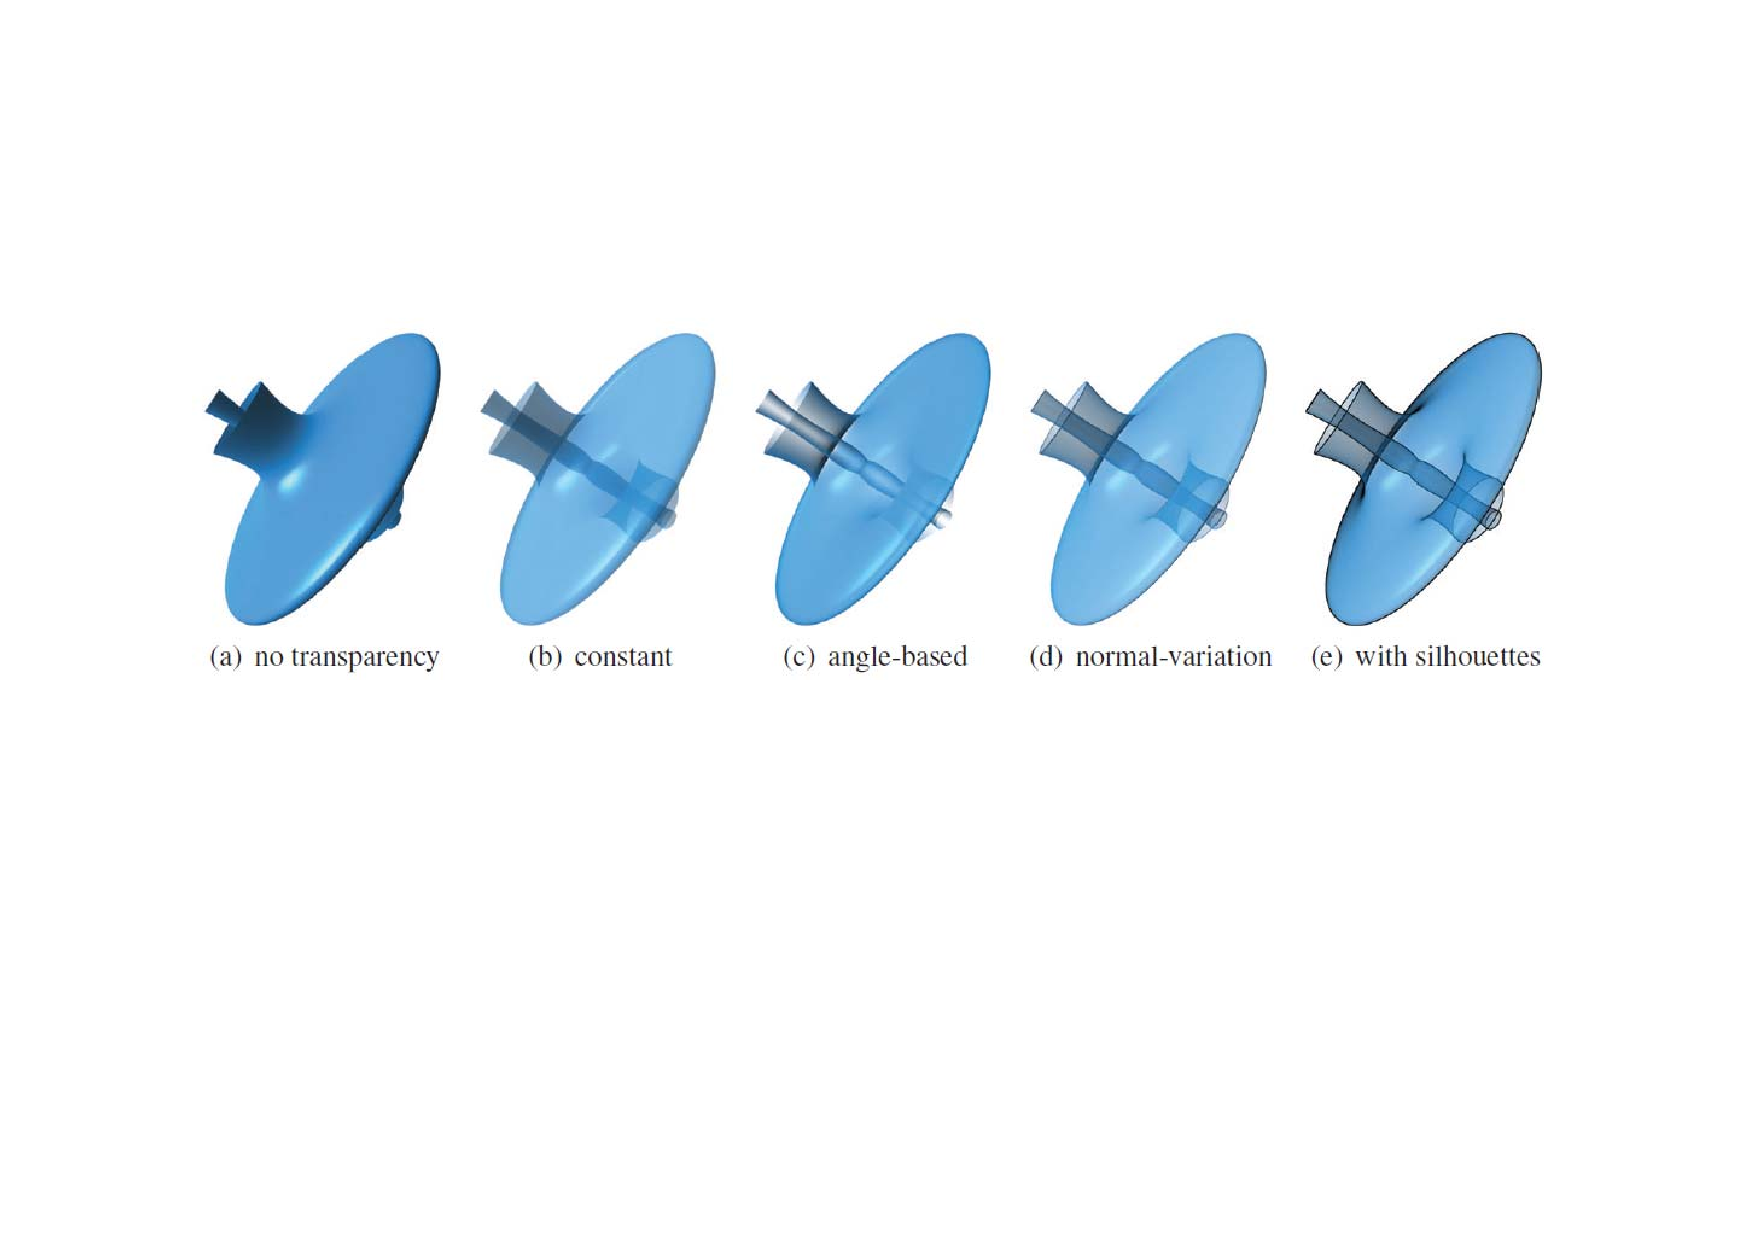
\includegraphics[width=0.9\textwidth,page=1]{img/11_transparency_methods}
\end{figure}

\begin{align*}
 \text{Angle based: }\qquad \alpha_\text{view} &= {2\over \pi} \arccos(N\cdot V)\\
 \text{Normal variation: }\qquad \alpha_\text{view} &= \left(
     \left( {\delta N_z \over \delta i}\right)^2
     +
     \left( {\delta N_z \over \delta j}\right)^2
 \right)^{\gamma/2}
\end{align*}

Normal variation approximates curvature and makes thinnest tubes most opaque.

Illustrators have numerous techniques for rendering of surfaces and textures. 




































